


%-------------------------

\newpage

%\section[From Paris to Zhuhai][De Paris à Zhuhai]{From Paris to Zhuhai}{De Paris à Zhuhai}
\section{From Paris to Zhuhai}{De Paris à Zhuhai}

\label{sec:casestudies}

%-------------------------


Nous développons dans cette section des cas d'étude géographique à l'échelle métropolitaine\comment[FL]{sens ?}, que nous choisissons très différents pour montrer la diversité des situations possibles\comment[FL]{pourquoi cet objectif, par ailleurs imprecis ?} mais aussi les motifs récurrents généraux qui pourraient se dégager. Il s'agit de la métropole du Grand Paris, et de la mega-région urbaine du Delta de la Rivière des Perles dans le sud de la Chine.


%-------------------------

%%%%%%%%%%%%%%%%%%%%%%%%
%\subsection[Greater Paris][Grand Paris]{Greater Paris: History and current Issues}{Le Grand Paris : histoire et enjeux}
\subsection{Greater Paris: History and current Issues}{Le Grand Paris : histoire et enjeux}


La région parisienne est une bonne illustration de la complexité des interactions entre réseaux de transports et territoires, au cours du temps et à l'échelle intermédiaire d'une région métropolitaine globalement monocentrique.\comment[FL]{faire plusieurs phrases} \cite{gilli2005bassin} rappelle l'importance de l'hinterland du Bassin Parisien et l'importance de ne pas considérer l'hypercentre de manière isolée. Si la moyenne couronne\comment[FL]{sens ?} possède un certain niveau de polycentricité\comment[FL]{sens ?}, notamment grâce à l'effet des villes nouvelles\comment[FL]{?} qui sont d'importants pôles d'emplois locaux~\cite{berroir2005contribution} qui même s'il a rapidement divergé des intentions planificatrices\comment[FL]{de qui ? qu'est ce que cela signifie ?}~\cite{es119}, est bien réel, le Bassin Parisien étendu peut être également lu ayant un certains nombre de centres\comment[FL]{centres urbains ?} importants à une heure de Paris : Chartres, Orléans, Rouen, Reims et Lille grâce à la grande vitesse. Le rôle des différentes infrastructures de transport dans les différentes dynamiques économiques en Ile-de-France n'est pas trivial, comme le montre~\cite{PADEIRO201344} qui cherche à expliquer statistiquement la croissance de l'emploi entre 1993 et 2008 dans les moyennes et petites communes franciliennes en fonction de la proximité à une infrastructure : les effets dépendent à la fois du mode (autoroute ou aéroport) mais aussi du secteur économique considéré. Réciproquement, les développements successifs, généralement par ruptures\comment[FL]{def}, que nous détaillerons par la suite, sont liés à des dynamiques de planification\comment[FL]{sens ?} et des processus de gouvernance\comment[FL]{sens ?} qu'il convient de comprendre de manière intégrée\comment[FL]{?}. La métropole parisienne, qu'on désignera par \emph{Grand Paris}\comment[FL]{que veux tu dire par cela ?}, et sa région d'influence élargie\comment[FL]{c'est flou}, témoignent ainsi de relations complexes entre territoires et réseaux.




\paragraph{Governance}{Gouvernance}

\cite{gilli2009paris} propose en 2009 un diagnostic de la situation institutionnelle de la région parisienne, et des pistes pour une approche couplée entre gouvernance et aménagement. La préfiguration de ``l'instauration d'un acteur collectif métropolitain'' correspond à la métropole du Grand Paris qui sera inaugurée 7 ans plus tard, puisque le conseil métropolitain est mis en place fin 2016.\comment[FL]{$\rightarrow$c'est trop tot pour parler de cela ; $\rightarrow$c'est incomplet (longues discussions anterieures sur ce type de demarche)} Son effectivité concrète reste quasi-nulle au moment de l'écriture, confirmant une certaines inertie des structures de gouvernance, qui a nécessairement un impact sur celle des réseaux de transport\comment[FL]{phrase naive}. La mise en place de ce nouveau niveau de gouvernance a été disséquée plus récemment toujours par~\cite{gilli2014gouverner}, où il la situe dans un contexte plus large socio-économique et urbain\comment[FL]{c'est flou}, en quelque sorte un diagnostic territorial qui explique certains aspects de ce besoin de mutation\comment[FL]{la notion de ``besoin'' de mutation est assez obscure\ldots}. En perte de vitesse sur le plan de l'aménagement, mais aussi sur le plan social au vu d'inégalités socio-économiques locales très fortes, la métropole a besoin de se réinventer, et se nouveau souffle se cristallise naturellement dans le Grand Paris, c'est à dire ``l'avenir de Paris est sa banlieue''\comment[FL]{de qui est cette citation ?}. Cette initiative se concrétise par la convergence d'une auto-organisation des élus locaux, et d'une redéfinition du rôle de l'état, voulue centralisatrice jusqu'en 2012 puis laissant la place libre à la gouvernance métropolitaine avec le nouveau gouvernement, même si les projets lancés et les financements restent les mêmes dans les grandes lignes : le projet du Grand Paris Express est un compromis entre la solution voulue par l'état et celle poussée par la région. Suivant~\cite{desjardins2016grand}, si la structure de gouvernance métropolitaine est aujourd'hui toujours relativement impuissante, et si l'oubli de l'aspect social du développement métropolitain est toujours très présent, ces mutations témoignent toutefois d'un changement structurel profond dans l'organisation de la région.




\paragraph{Grand Paris Transportation Network}{Réseau de Transport du Grand Paris}

L'histoire du développement du réseau de transport de la métropole francilienne est rappelée dans~\cite{beauguitte:halshs-01068589}. La particularité centralisatrice française a conduit à une structure particulière du réseau ferré à l'échelle nationale, mais aussi à celle régionale. La domination de Paris a en effet fortement marqué la structuration du réseau de transport au cours des différentes périodes historiques où il a subit des évolutions conséquentes. Avant 1975, la distribution de l'accessibilité est clairement centralisée et le centre de Paris fortement congestionné. La mise en place du réseau RER entre 1975 et 1990, même si elle ne suit pas la volonté initiale de Delouvrier qui comprenait un plus grand nombre de branches transversale, permet la concrétisation d'un certain niveau de polycentrisme grâce à la construction conjointe des Villes Nouvelles. La période qui suivra jusqu'à aujourd'hui visera surtout à des désenclavements, mais aucun changement majeur d'accessibilité n'est observé. Les schémas directeurs successifs, qui aboutiront au SDRIF de 2013~\cite{sdrif2013}, préfigurent le futur réseau du Grand Paris Express, qui aura un impact crucial en terme de cohésion territoriale en favorisant les liaisons de banlieue à banlieue qui sont les plus problématique dans le réseau actuel. De plus, le schéma se veut pensé de manière intégrée, par densification autour des gares et articulation des opérations d'aménagement et les nouvelles infrastructures. Cet aspect d'intégration des réseaux dans les territoires et des territoires par les réseaux se retrouve bien dans la communication publique de l'Autorité Organisatrice des Transports (ancien STIF, devenu Ile-de-France Mobilités)\footnote{voir l'actualité du 4 octobre 2017 sur \texttt{https://www.iledefrance-mobilites.fr/actualites/un-reseau-de-transports-qui-grandit/} qui souligne que ``\textit{Avec 29 km de réseau supplémentaires et l’ouverture de 28 points de desserte, les territoires se rapprochent}'', témoignant de l'importance de l'accessibilité pour les territoires, notion par ailleurs floue. Les mêmes orientations de discours se retrouvent pour les différents projets d'extension ou de construction de nouvelles lignes.}




\paragraph{Impact of the Grand Paris Express}{Impact du Grand Paris Express}

\bpar{
The metropolitan region of Paris is currently undergoing large mutations, with the institution of a metropolitan governance and new transportation infrastructures for example. The construction of a ring underground allowing suburbs to suburbs links is a rather ancient need, and lead to several proposals on which the State and the Region have been in conflict around 2010~\cite{desjardins2010bataille}. The \emph{Arc Express} project~\cite{stif2007arc} advocated by the Region and focused towards territorial equity can be contrasted with initial proposals for a \emph{Réseau du Grand Paris} aimed at linking ``excellence clusters'' despite a potential tunnel effect. The solution finally chosen (see the last \emph{Schéma Directeur}~\cite{sdrif2013}) is a compromise between the two and allows a rebalancing of accessibility between the west and the east~\cite{beaucire2013grand}.
}{
La région métropolitaine de Paris est en train de connaître de grandes mutations, avec la mise en place d'une gouvernance métropolitaine et de nouvelles infrastructures de transport par exemple. La construction d'un réseau de métro en rocade permettant des liaisons de banlieue à banlieue est un besoin ancien, et a mené à plusieurs propositions sur lesquelles se sont opposés l'Etat et la Région au tournant des années 2010~\cite{desjardins2010bataille}. Le projet Arc Express~\cite{stif2007arc}, porté par la Région et plus axé sur une égalité des territoires, contrastait avec les propositions initiales de Réseau du Grand Paris visant à relier des ``clusters d'excellence'' en dépit d'un possible effet tunnel. La solution finalement adoptée (voir le dernier schéma directeur \cite{sdrif2013}) est un compromis et permet un rééquilibrage est-ouest de l'accessibilité~\cite{beaucire2013grand}.
}

Les impacts immédiats d'une nouvelle de transport en terme d'accessibilité concernent généralement des territoires bien plus larges que les zones où la ligne et ses stations sont implantées : les motifs d'accessibilité sont dus aux propriétés topologiques du réseau et celles-ci sont fortement discontinues en fonction de la structure du graphe. Illustrons le cas des lignes du Grand Paris Express et de leur impact direct sur l'accessibilité régionale. La Fig.~\ref{fig:casestudies:gpe} cartographie les gains de temps moyens permis par ce projet sur les départements métropolitains (75, 92, 93 et 94)\footnote{voir la section~\ref{sec:grandparisrealestate} pour le détail de la méthodologie de calcul.}, avec le tracé le plus récent pour l'ensemble des lignes. On observe, conformément à l'analyse de~\cite{beaucire2013grand}, un rééquilibrage des différentiels d'accessibilité entre Est et Ouest. A distance égale du centre, l'accessibilité temporelle moyenne est plus élevée pour la Seine-Saint-Denis et le Val-de-Marne que pour les Hauts-de-Seine. La carte des gains temporels moyens montre les gains plus grands également pour ces deux départements. Des communes socio-économiquement défavorisées comme Aulnay sont bénéficiaires des plus grands gains de temps. La ligne 16 est en effet précisément dédiée au désenclavement du nord-est de la Seine-Saint-Denis~\cite{desjardins2016grand}. La création de liaisons de banlieue à banlieue est un aspect majeur de ce désenclavement et est voulue comme un moteur de l'émergence de nouvelles centralités, vers une métropole toujours plus polycentrique, dans la lignée de la politique d'aménagement des villes nouvelles, pour ne plus parler de proche banlieue mais de quartiers faisant partie intégrante du Grand Paris. Les effets peuvent cependant être mitigés selon les zones : \cite{l2013grand} montre que le Grand Paris Express induira un accès direct à un plus grand nombre d'emplois pour un nombre significatif de chômeurs en petite couronne, mais que les écarts avec la grande couronne seront accentués et qu'il existe des risques de décrochage de certaines communes lointaines mal desservies. L'un des enjeux cruciaux pour la construction du Grand Paris est de veiller à ne pas obtenir une métropole à plusieurs vitesses, et de tirer parti de la connectivité accrue à plusieurs échelles (internationale, nationale, régionale, métropolitaine) pour réduire les inégalités territoriales plutôt que les accroitre. Le nouveau réseau semble contribuer à cette dynamique, sous condition d'un développement territorial coordonné, permettant la concrétisation des gains immédiats d'accessibilité en terme de transformation territoriale. Il n'existe pas de méthode pouvant prévoir celle-ci de manière sûre comme mous l'avons déjà développé. L'un des enjeux de notre travail par la suite sera de clarifier empiriquement des situations dans lesquelles des dynamiques fortement couplées relevant de cette problématique pourront être mises en évidence puis à travers des modèles d'isoler des processus et des conditions permettant telle ou telle situation.



%%%%%%%%%%%%%%%%%%%
\begin{figure}
	%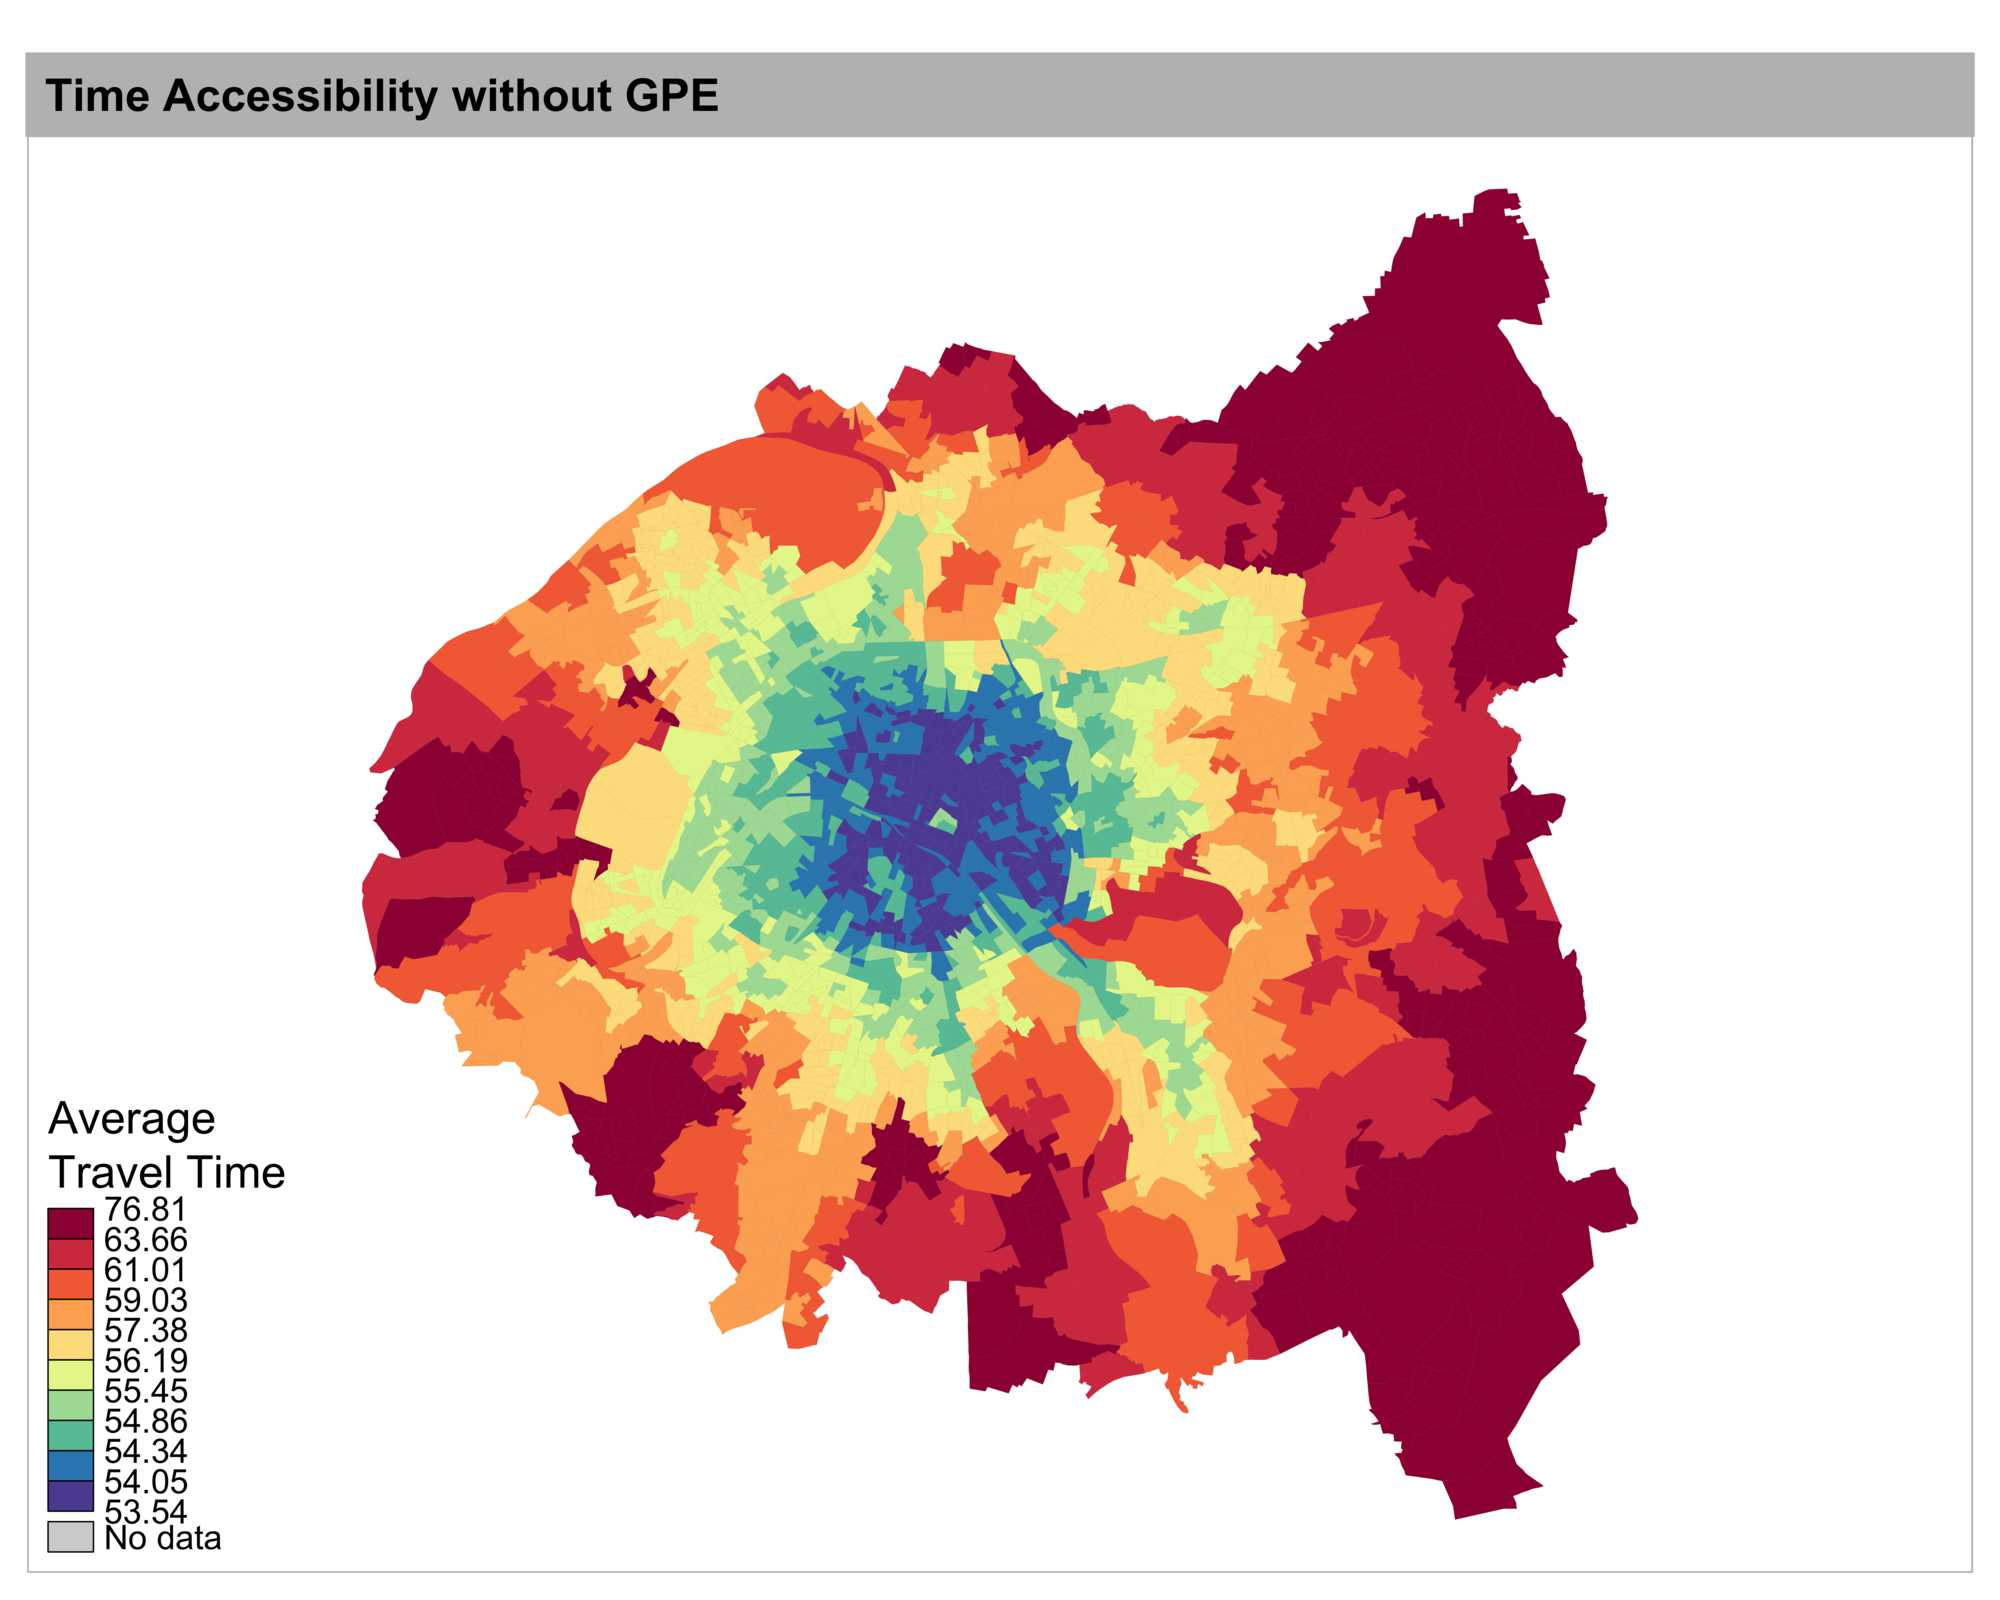
\includegraphics[width=0.8\linewidth]{Figures/CaseStudies/timeaccess_metropole}\\
	%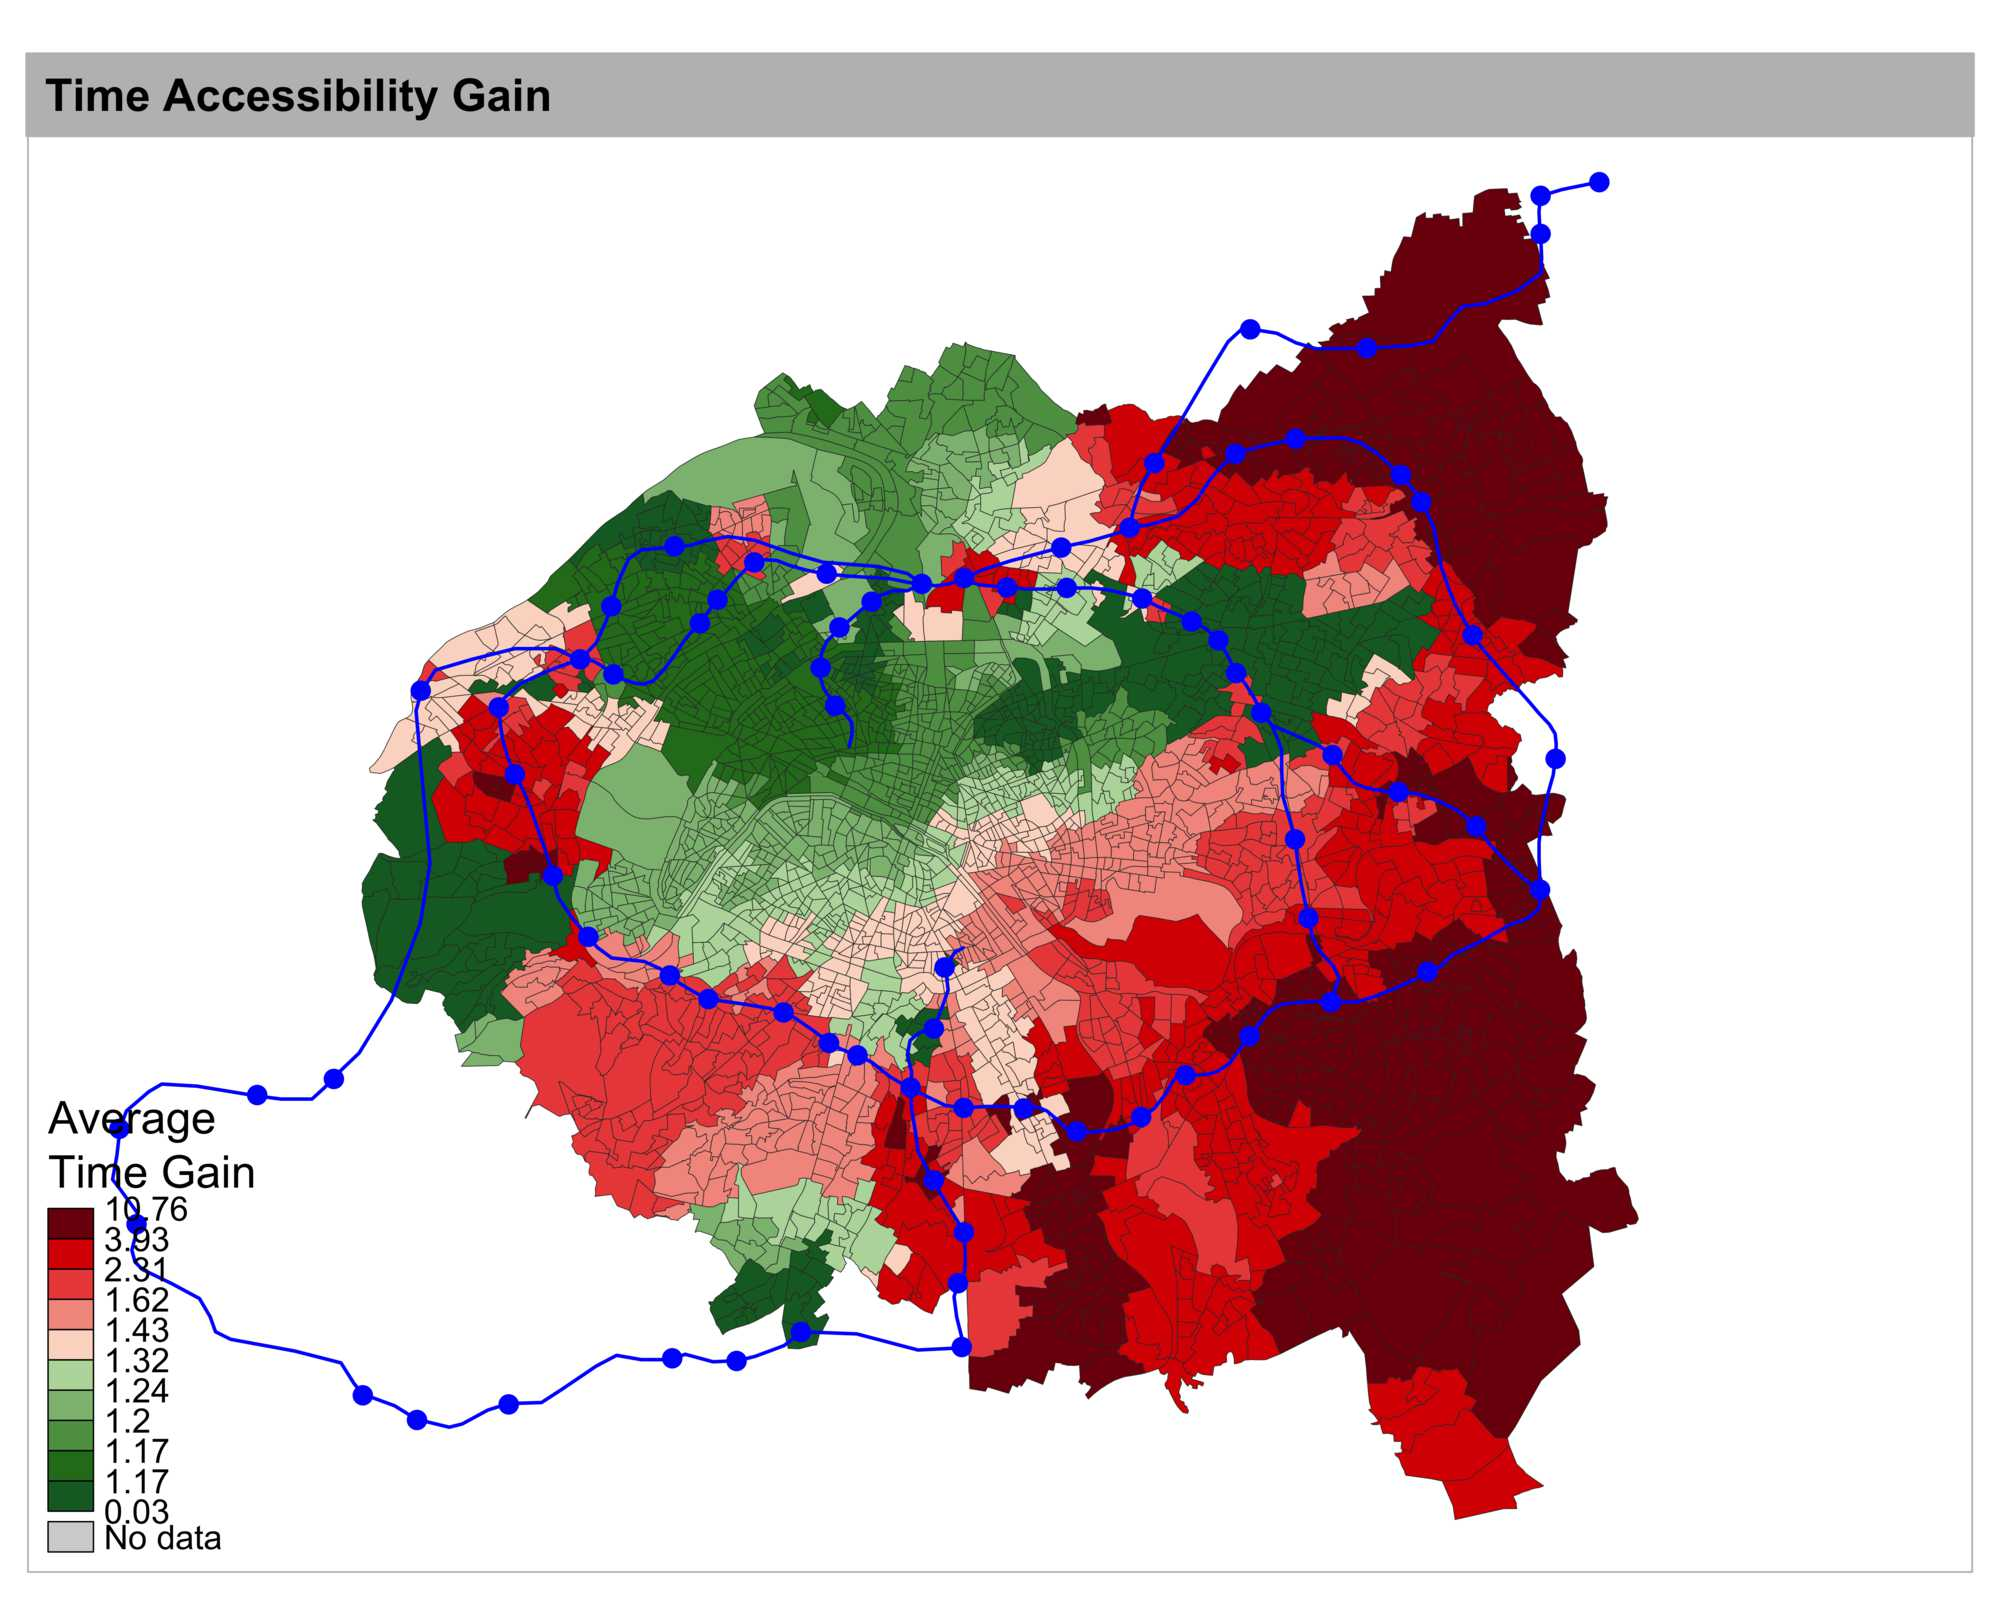
\includegraphics[width=0.8\linewidth]{Figures/CaseStudies/timegain_metropole}
	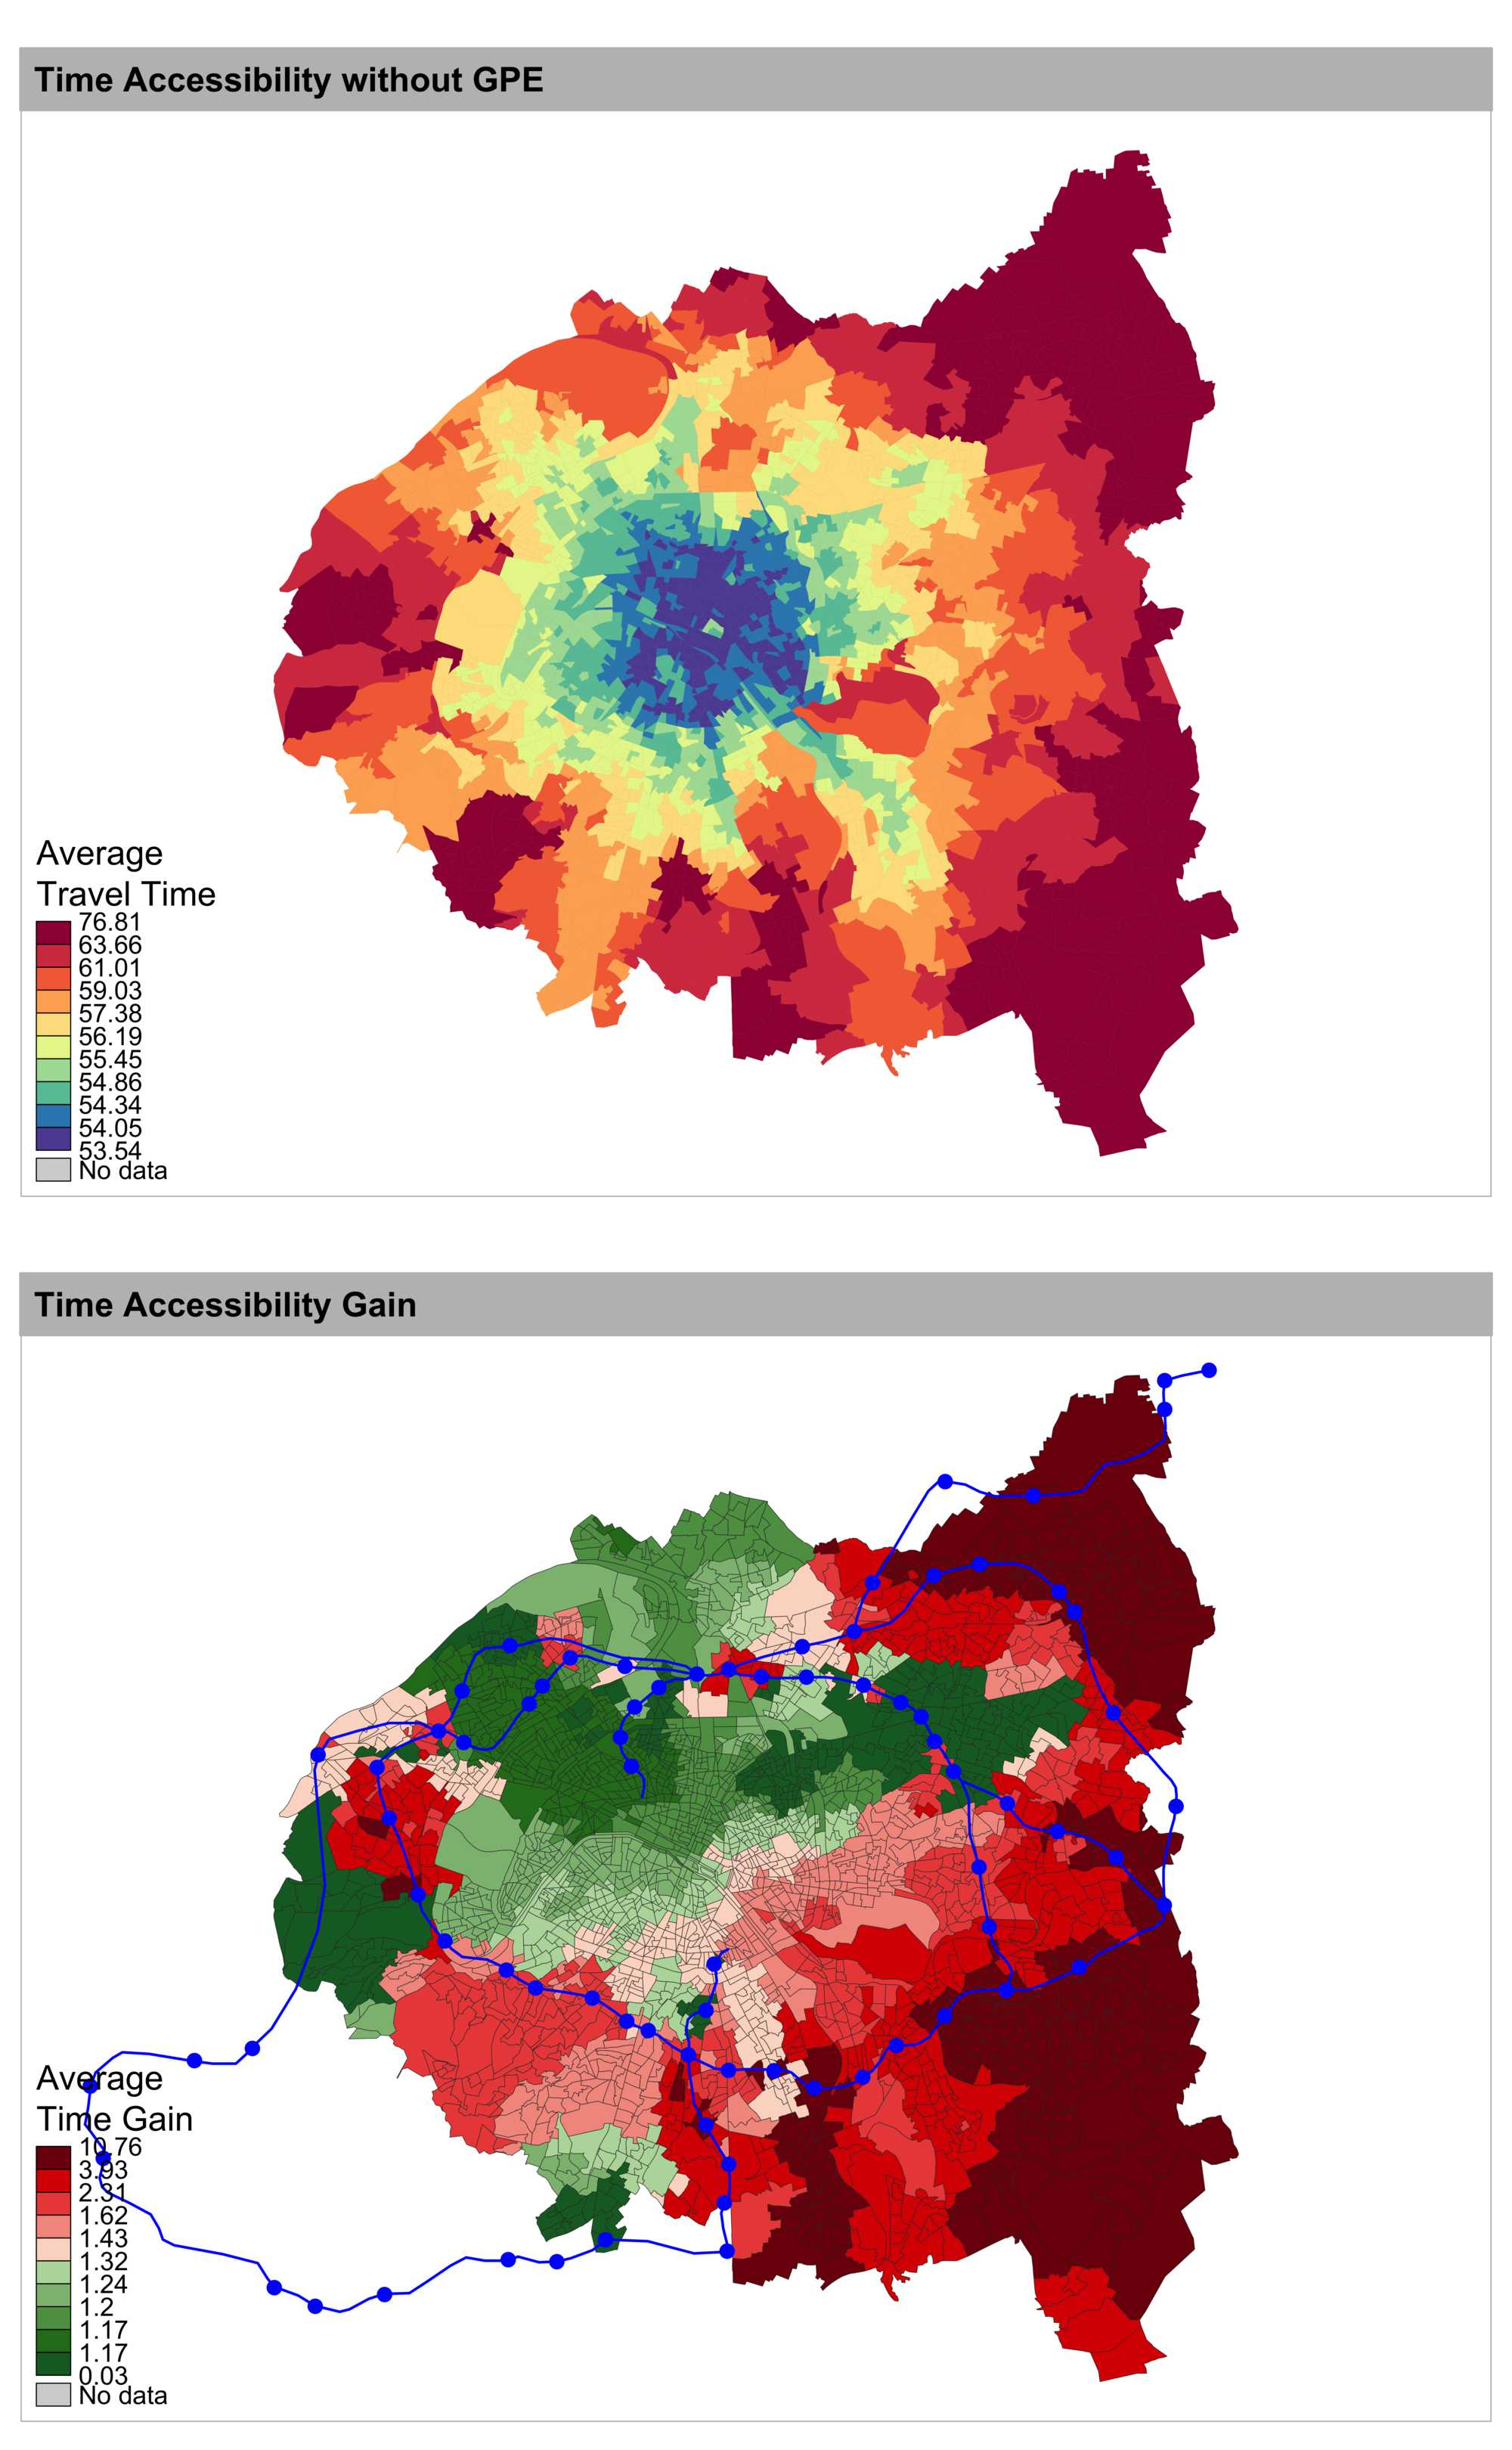
\includegraphics[width=\linewidth]{Figures/Final/1-2-1-fig-casestudies-gpe.jpg}
	\caption[Impact of \emph{Grand Paris Express}][Impact du Grand Paris Express]{\label{fig:casestudies:gpe}}{\textbf{Impact des lignes du GPE sur l'accessibilité temporelle.} \textit{(Haut)} Temps moyen de trajet vers l'ensemble des communes d'Ile-de-France, par transports en commun uniquement, pour les départements métropolitains ; \textit{(Bas)} Gains de temps permis par l'ensemble des lignes du GPE, avec le trajet des lignes.\label{fig:casestudies:gpe}}
\end{figure}
%%%%%%%%%%%%%%%%%%%




\bpar{
Various aspects of territories are concerned by interactions with networks. In previous empirical studies, no socio-economic attributes of populations inhabiting the territory nor economic values for land and real estate was considered. Both are however crucial elements of territorial dynamics and are extensively studied in fields such as territorial analysis or urban economics : for example, \cite{homocianu:tel-00359302} studies households residential choices to understand land-use transportation interactions. We propose here to use a database of Real Estate transactions for Parisian region on the last 20 years, with 2 years temporal granularity and exact spatial coordinates. \cite{guerois2009dynamique} used it to make typologies of spatial dynamics of Parisian real estate.
}{
Des aspects très variés des territoires sont concernés par l'interaction avec les réseaux. Dans nos études précédentes, les aspects économiques et financiers du foncier et l'immobilier n'ont pas été considérés. Il s'agit cependant d'éléments cruciaux des dynamiques territoriales et sont étudiés de manière intensive dans des champs comme l'analyse territoriale ou l'économie urbaine : par exemple, \cite{homocianu:tel-00359302} étudie les choix résidentiels des ménages pour comprendre les interactions entre usage du sol et transport. Nous proposons ici d'utiliser entre autres une base de données de transactions immobilières pour la région parisienne sur les 20 dernières années, avec une granularité temporelle de 2 ans et coordonnées spatiales exactes. \cite{guerois2009dynamique} l'utilise par exemple pour établir une typologie des dynamiques spatiales du marché immobilier parisien.
}


\bpar{
We propose to study the relations between accessibility differentials for each project, with variables linked to real estate and socio-economic variables. Indeed, the links between new lines and real estate value evolution are sometimes dramatic~\cite{damm1980response}. 
}
{
Cette étude plus précise peut être comprise comme une recherche de signes précurseurs de rupture de potentiels du réseau: en effet, si des dynamiques territoriales intrinsèques anticipent l'arrivée d'une nouvelle station de transports en commun, les implications seront bien différentes du cas où celle-ci conduit ces variables après sa construction. L'interprétation en termes ``d'effets structurants'' sera notamment très différente. Nous appliquons ici la méthode de causalités spatio-temporelles développée en~\ref{sec:causalityregimes}. Nous proposons d'étudier les relations entre différentiel d'accessibilité pour chaque projet, et variables liées au foncier (transactions immobilières) et socio-économiques. En effet, les liens entre nouvelles lignes et évolution du foncier sont parfois remarquables~\cite{damm1980response}.
}

\comment{sur les anticipations des acteurs : \cite{carrouet:hal-00980002} }


\cite{guerois2009dynamique} : bulles immobilières locales ?


\bpar{
Data for real estate transactions are contained within the BIENS database (\emph{Chambre des Notaires d'Ile de France}, proprietary database). The number of transactions that can be used after cleaning is 862360, distributed across all IRIS areas (basic census units in France), for a temporal span covering the years 2003 to 2012 included. The data at the IRIS level for population and income (median income and Gini index) come from INSEE. Network data have been vectorialized from projects maps (see figure~\ref{fig:projects} for the different projects). Travel times are computed by public transportation only, with standard values for average speeds of different modes (RER 60km.h\textsuperscript{-1}, Transilien 100km.h\textsuperscript{-1}, Metro 30km.h\textsuperscript{-1}, Tramway 20km.h\textsuperscript{-1}). The travel time matrix is computed from all the centroids of IRIS to all the centroids of \emph{Communes} (above aggregation level). These are linked to the network with abstract connectors to the closest station, with a speed of 50km.h\textsuperscript{-1} (travel by car). Analysis are implemented in R~\cite{rcoreteam} and all data, source code and results are available on an open git repository\footnote{At\\\texttt{https://github.com/JusteRaimbault/CityNetwork/tree/master/Models/SpatioTempCausality/GrandParis}. Data for the BIENS database are given only at the aggregated level of IRIS and for price and mortgage variables, for contractual reasons closing the database.}.
}{
Les données des transactions immobilières sont fournies par la base BIENS (Chambre des Notaires d'Ile de France, base propriétaire). Le nombre de transactions utilisables après nettoyage est de 862360, se répartissant sur l'ensemble des IRIS, pour une plage temporelle couvrant de 2003 à 2012 incluses. Les données par IRIS pour population et revenu (revenu médian et indice de Gini) proviennent de l'INSEE. Les données de réseau ont été vectorialisées à partir des cartes des projets (voir Fig.~\ref{fig:projects} pour les projets). Les temps de trajets sont calculés par transport en commun uniquement, avec des valeurs standard pour les vitesses moyennes des différents modes (RER 60km.h\textsuperscript{-1}, Transilien 100km.h\textsuperscript{-1}, Metro 30km.h\textsuperscript{-1}, Tramway 20km.h\textsuperscript{-1}). La matrice des temps est calculée depuis l'ensemble des centroïdes des IRIS vers l'ensemble des centroïdes des communes. Ceux-ci sont reliés au réseau par des connecteurs à la gare la plus proche, de vitesse 50km.h\textsuperscript{-1} (trajet en voiture). Les analyses sont implémentées intégralement en langage R~\cite{rcoreteam} et l'ensemble des données, du code source et des résulats sont disponibles sur un dépôt git ouvert\footnote{A l'adresse\\\texttt{https://github.com/JusteRaimbault/CityNetwork/tree/master/Models/SpatioTempCausality/GrandParis}. Les données de la base BIENS ne sont fournies que de manière agrégée à l'IRIS et pour les variables de prix et de crédit, pour des raisons de fermeture contractuelle de la base brute.}.
}



%%%%%%%%%%%%%%%
\begin{figure}
%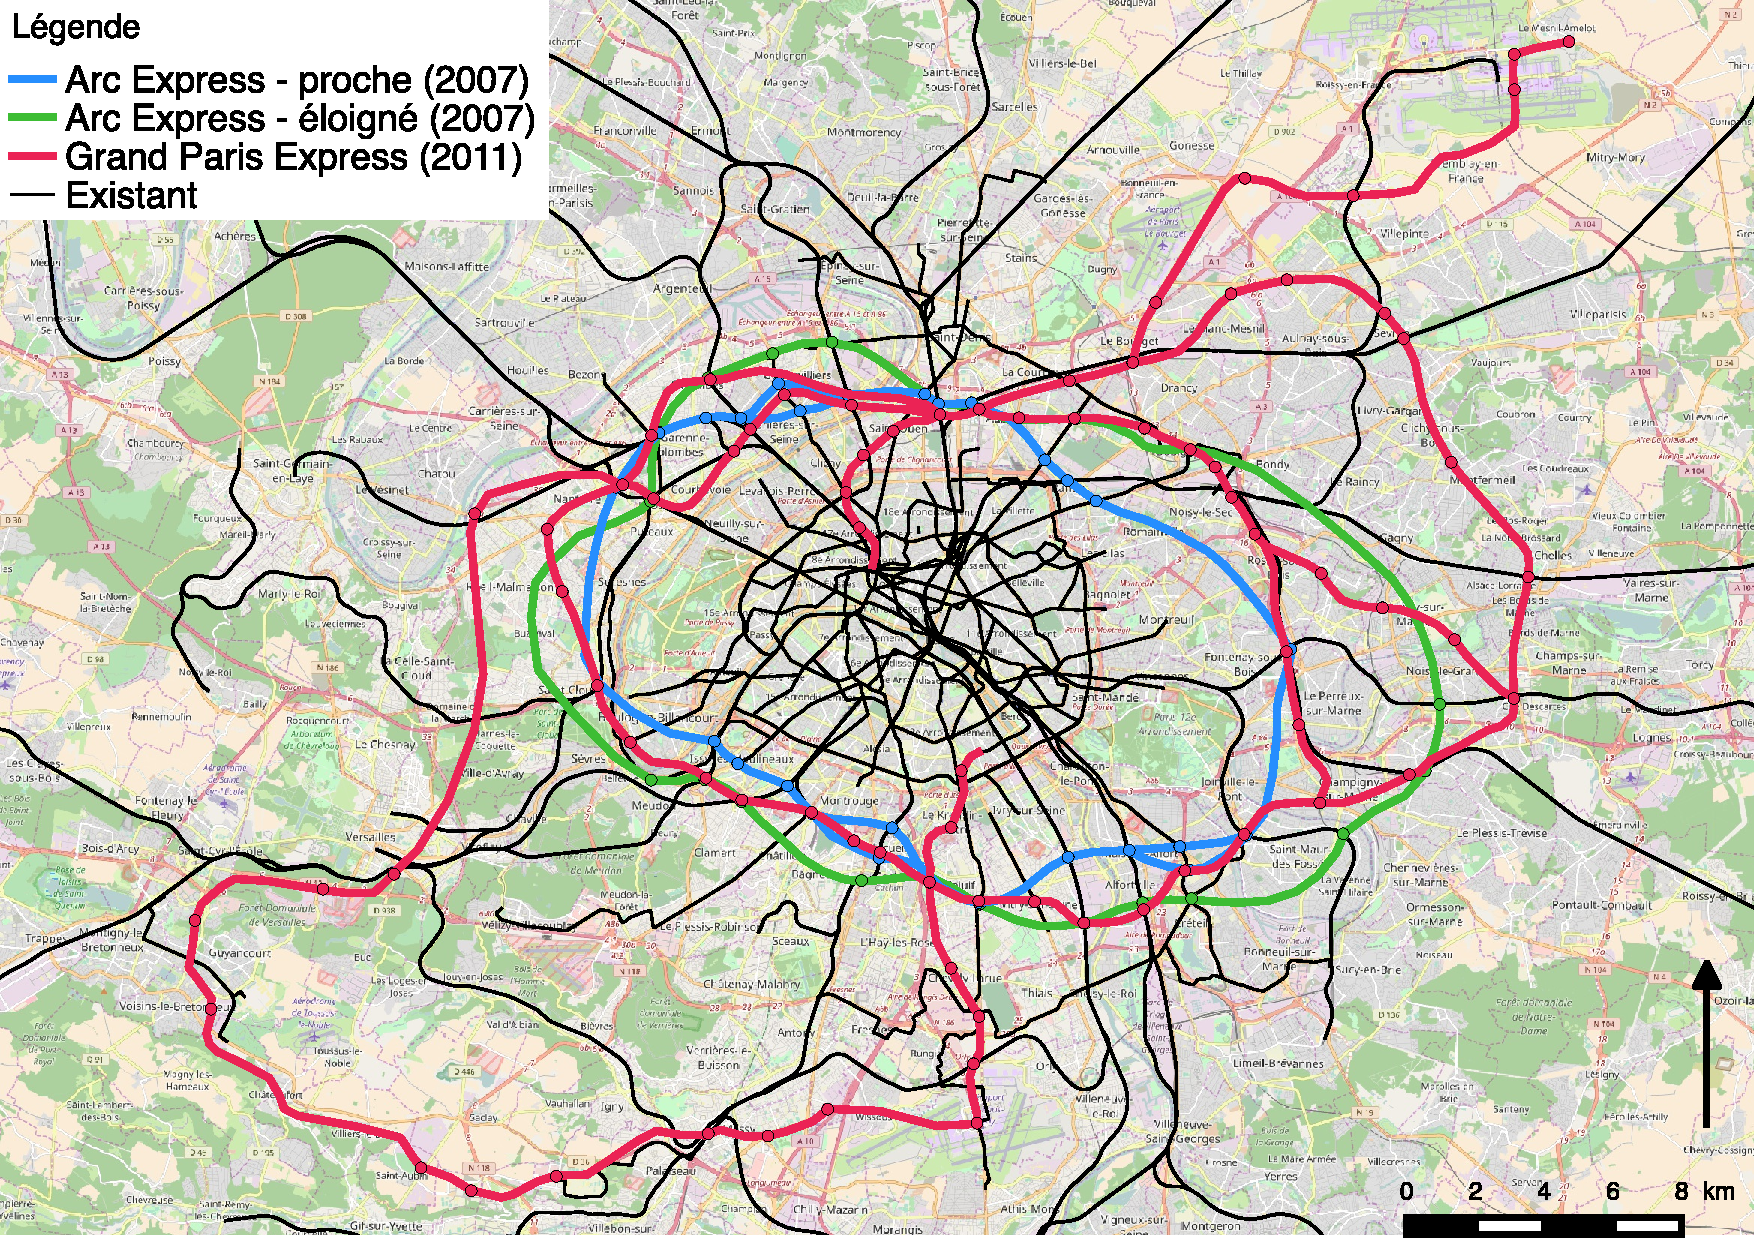
\includegraphics[width=\linewidth]{Figures/GrandParisRealEstate/reseaux}
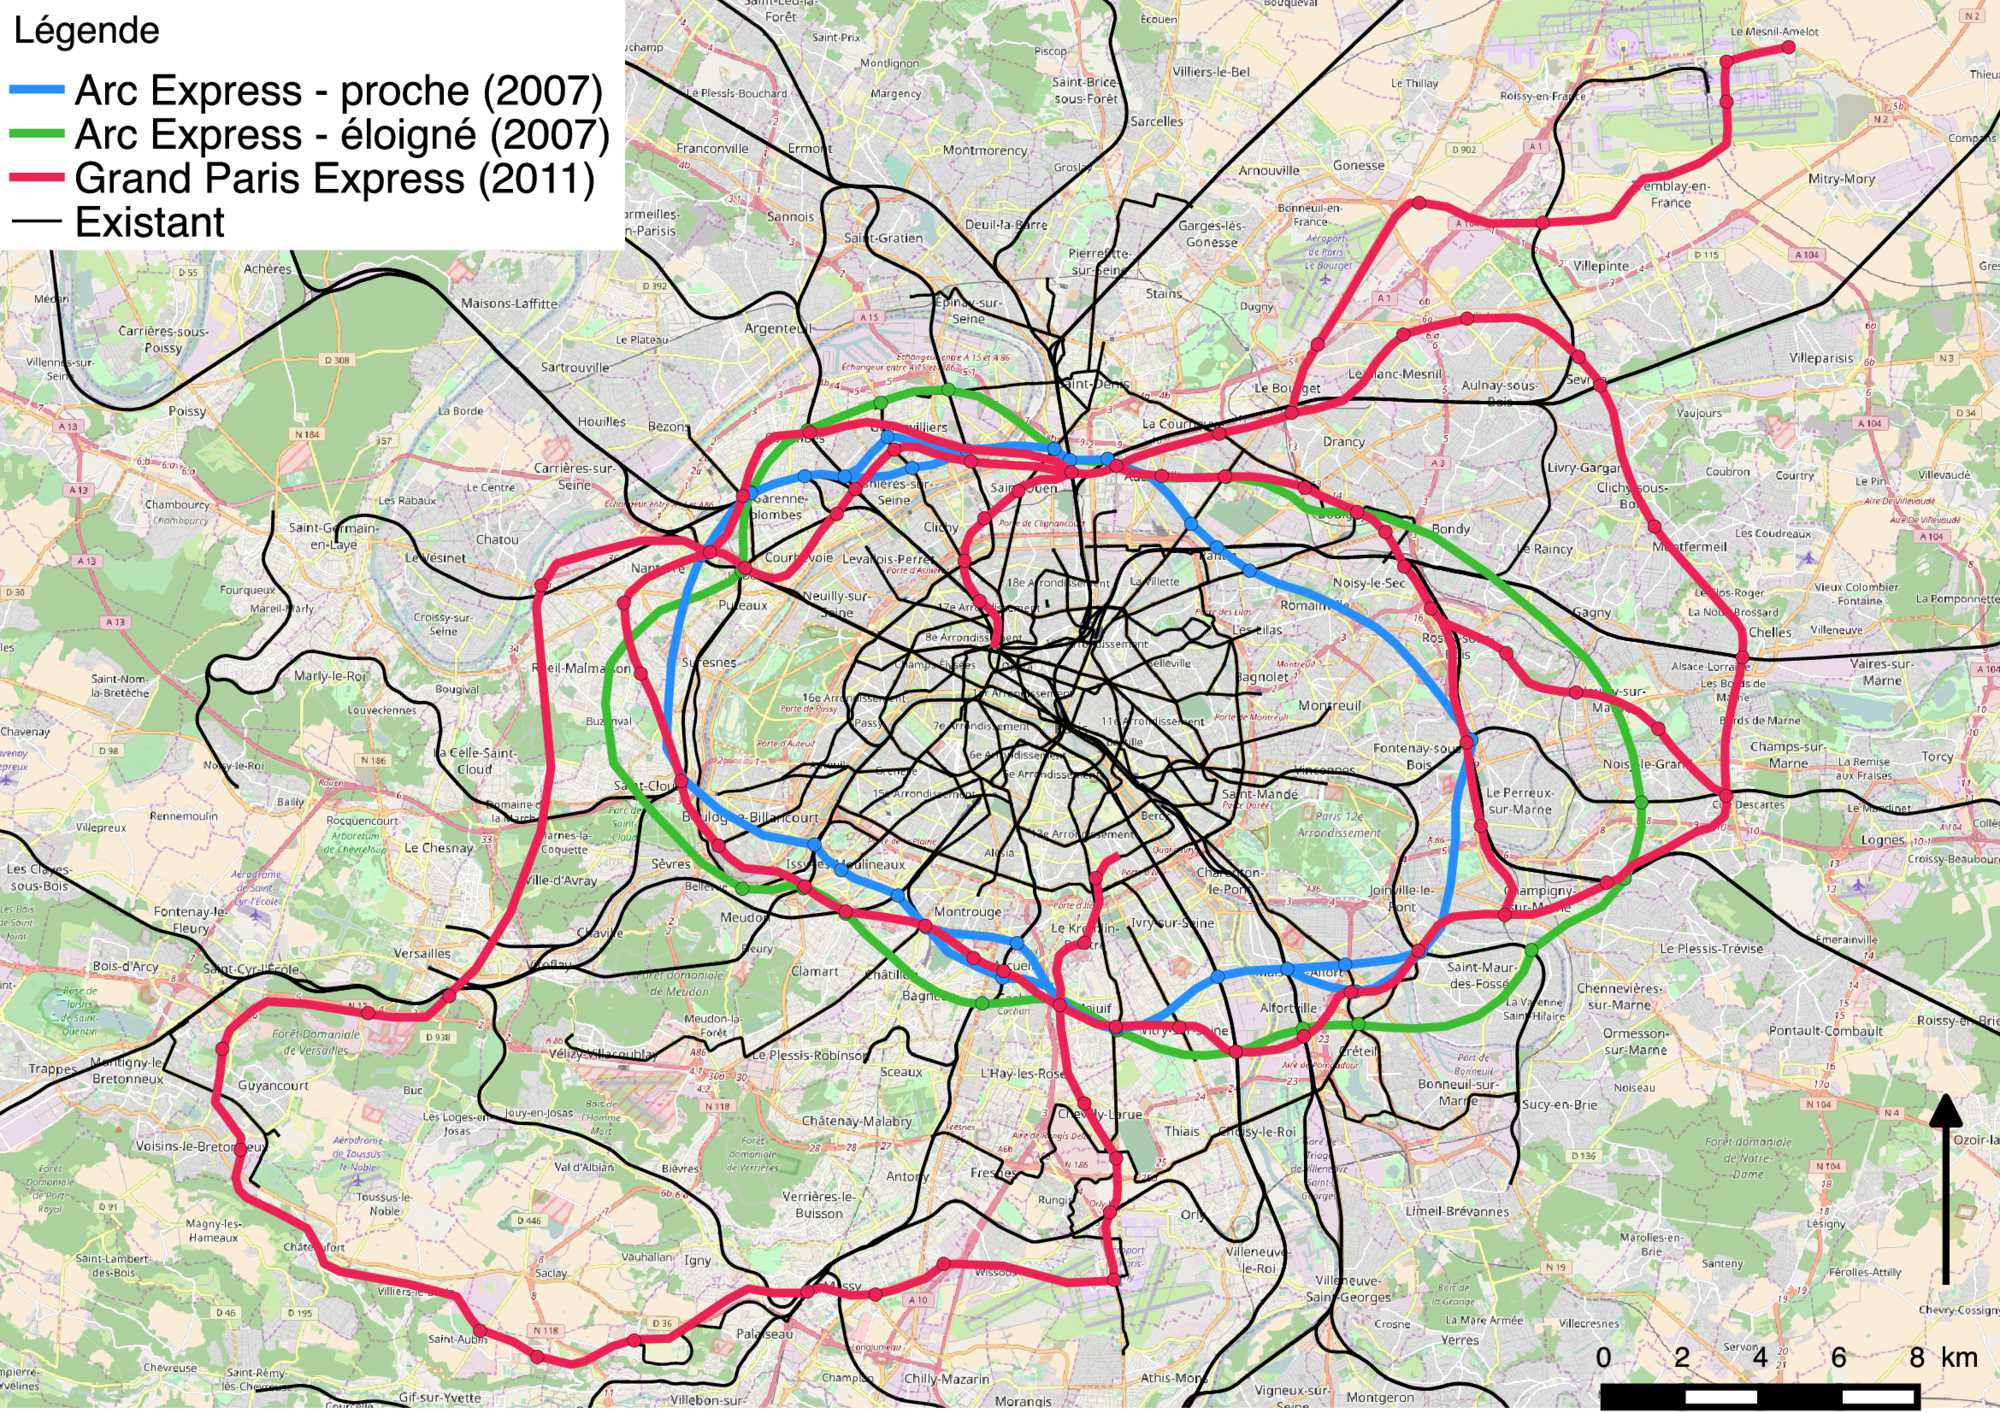
\includegraphics[width=\textwidth]{Figures/Final/1-2-1-fig-casestudies-projects.jpg}
\caption[][Projets de transport successifs du Grand Paris]{\textbf{Successive transportation network projects for the Grand Paris metropolitan area.} We show the two alternatives for the \emph{Arc Express} project elaborated by the Region, and the \emph{Grand Paris Express} (GPE) advocated by the State. The \emph{Réseau du Grand Paris}, a precursor for GPE, is not shown here for visibility reasons because of its proximity with it.\label{fig:projects}}{\textbf{Projets de transport successifs de la métropole du Grand Paris.} Nous montrons les deux alternatives du projet Arc Express porté par la région, et le Grand Paris Express (GPE) porté par l'état. Le Réseau du Grand Paris, précurseur du GPE, n'est pas montré ici pour des raisons de visibilité à cause de sa proximité avec celui-ci.\label{fig:casestudies:projects}}
\end{figure}
%%%%%%%%%%%%%%%


\bpar{

We compute for each project accessibility differentials $\Delta T_i$ in average travel time from each IRIS, in comparison with the network without the project. Average travel time accessibility is defined as $T_i = \sum_k \exp{-t_{ik}/t_0}$ with $k$ \emph{Communes}, $t_{ik}$ travek time, and $t_0$ a decay parameter. To each project is associated a date\footnote{2006 for \emph{Arc Express}, 2008 for \emph{Réseau du Grand Paris} and 2010 for \emph{Grand Paris Express}}, corresponding roughly to the mature announcement of the project. It stays a bit arbitrary as it is difficult on the one hand to determine precisely as a planning project does not emerge from nothing in one day, and one the other hand it may correspond to different realities of learning about the project by economic agents (we do therefore the limiting but necessary assumption of a diffusion of information for the majority of agents in a time smaller than a year). We study the lagged correlations of this variable with the variations $\Delta Y_{ij}$ of the following socio-economic variables: population, median income, Gini index for income, average price of real estate transactions and average value of real estate mortgages. A Fisher test is done for each estimation and the value is set to 0 if it is not significant ($p<0.05$ in a classical manner). The study with generalized accessibility in the sense of Hansen has also been conducted but is less interesting as it has a very low sensitivity to the mobility component (network and decay) compared to the variables themselves. It informs therefore only on relations between these and is not presented here. We show in figure~\ref{fig:empiricalres} the results for all networks and variables. It is first remarkable to note the presence of significant effects for all variables. Lower values for the parameter $t_0$ give correlations higher in absolute value, unveiling a possible higher importance of local accessibility on territorial dynamics. The behavior of population shows a clearly detached peak corresponding to 2008, what suggests an impact of the older project \emph{Arc Express} on population growth, the effect of other projects would then be spurious from their proximity in the most important branches. It would imply that areas where they are fundamentally different such as \emph{Plateau de Saclay} are less sensitive to transportation projects, what would confirm the artificial planned aspect of the development of this territory. Concerning income, we observe a similar behavior but in a negative way, what would imply a decrease of wealth linked to the increase of accessibility, however accompanied by a decrease of inequalities. Finally, real estate prices are as expected driven by the potential arrival of new networks. This effect disappear after two years for the \emph{Grand Paris Express}, suggesting a temporal speculation bubble. We demonstrate thus the existence of complex lagged correlation links, that we call causalities in this sense, between territorial dynamics and anticipated dynamics of networks. A finer understanding of working processes is beyond the scope of this paper and would imply for example qualitative fieldwork or targeted case studies. This example shows however the operational potentialities of our method on a real case study.
}{
Nous calculons pour chaque projet, le différentiel $\Delta T_i$ d'accessibilité en temps moyen de trajet à partir de chaque IRIS en comparaison à celui dans le réseau sans le projet, défini par $T_i = \sum_k \exp{-t_{ik}/t_0}$ avec $k$ communes, $t_{ik}$ temps de trajet, et $t_0$ paramètre d'atténuation. A chaque projet est associée une date\footnote{2006 pour Arc Express, 2008 pour le Réseau du Grand Paris, 2010 pour le Grand Paris Express}, correspondant environ à l'année d'annonce mature du projet, restant toutefois arbitraire car difficile d'une part à déterminer précisément, un projet n'émergeant pas d'un coup du jour au lendemain, et d'autre part pouvant correspondre à des réalités différentes d'apprentissage du projet par les différents agents économiques (nous faisons donc l'hypothèse réductrice mais nécessaire d'une diffusion sur la majorité des agents dans un temps inférieur à l'année). Nous étudions les corrélations décalées de cette variable avec les variations $\Delta Y_{ij}$ des variables socio-économiques suivantes : population, revenu médian, indice de Gini des revenus, prix moyen des transactions immobilières et montant moyen des crédits immobiliers. Un test de Fisher est effectué pour chaque estimation, et la valeur est fixée nulle si celui-ci n'est pas significatif ($p<0.05$ de manière classique). L'étude avec accessibilité généralisées au sens de Hansen a également été menée mais moins intéressante car très peu sensible à la composante mobilité (réseau et atténuation) par rapport aux variables elle-même, informe uniquement sur des relations entre celles-ci et n'est donc pas présentée ici. Nous présentons en Fig.~\ref{fig:empiricalres} les résultats pour l'ensemble des réseaux et variables. Il est remarquable tout d'abord de noter l'existence d'effets significatifs pour l'ensemble des variables. Des valeurs plus basses du paramètre $t_0$ donnent des corrélations plus fortes en valeur absolue, révélant une possible plus grande importance de l'accessibilité locale sur les dynamiques territoriales. Le comportement de la population montre un pic très détaché correspondant à 2008, laissant supposer un impact du plus vieux projet d'Arc Express sur la croissance de la population, l'effet des autres projets serait alors fallacieux de par leur proximité dans les grands tronçons : cela impliquerait que les zones où ils diffèrent fondamentalement comme le Plateau de Saclay ne soient que très peu sensibles au projet de transport, ce qui confirmerait l'aspect artificiel planifié du développement de ce territoire. Concernant les revenus, on observe un comportement similaire mais négatif, ce qui impliquerait un appauvrissement lié à l'augmentation de l'accessibilité, mais qui semble toutefois s'accompagner d'une baisse des inégalités. Enfin, comme attendu les prix immobiliers sont tirés par l'arrivée potentielle des nouveaux réseaux, effet qui disparait à deux ans pour le Grand Paris Express, suggérant une bulle immobilière passagère. Nous démontrons ainsi l'existence de liens de correlations retardées complexes qu'on nomme causalités en ce sens, entre dynamiques territoriales et dynamiques anticipées des réseaux. Une compréhension plus fine des processus à l'oeuvre est au delà de la portée de cet article, car supposerait des études de terrain qualitatives, des études de cas ciblées, etc. Cet exemple illustre cependant le caractère opérationnel de notre méthode sur un cas d'étude réel.
}


%%%%%%%%%%%%%%%
\begin{figure}[h!]
%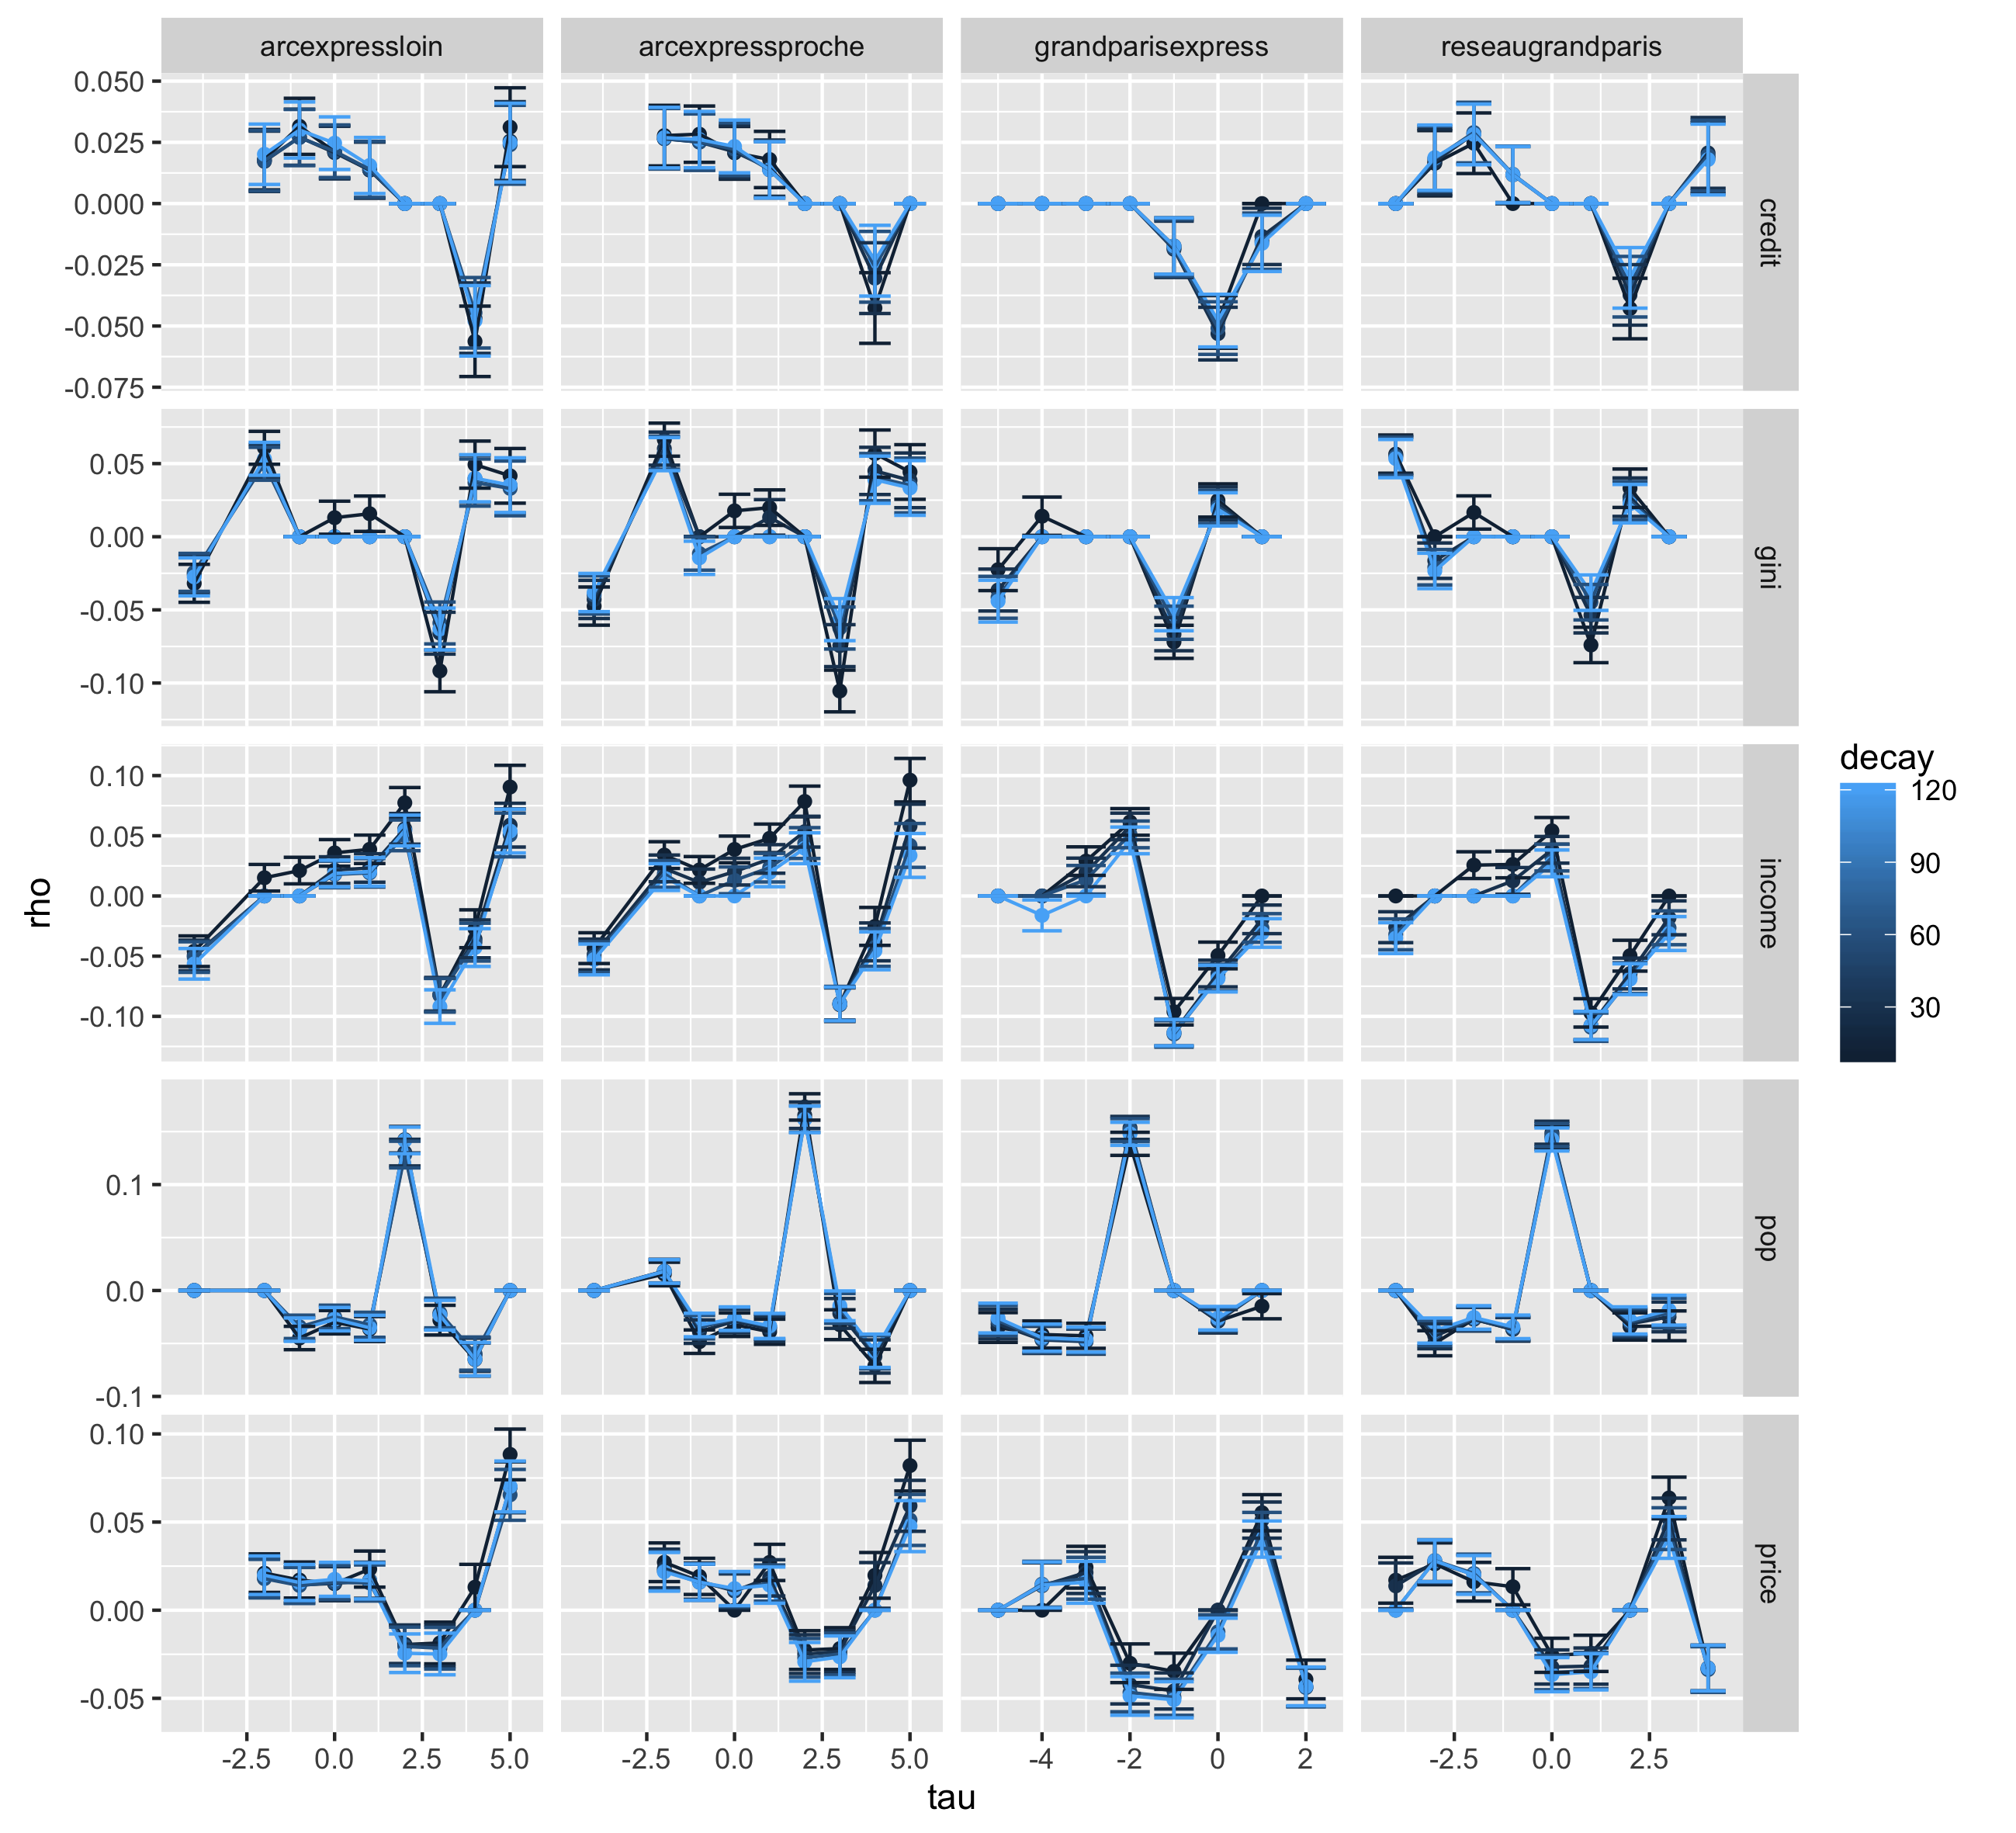
\includegraphics[width=\linewidth]{Figures/GrandParisRealEstate/laggedcorrs_times_allvars}
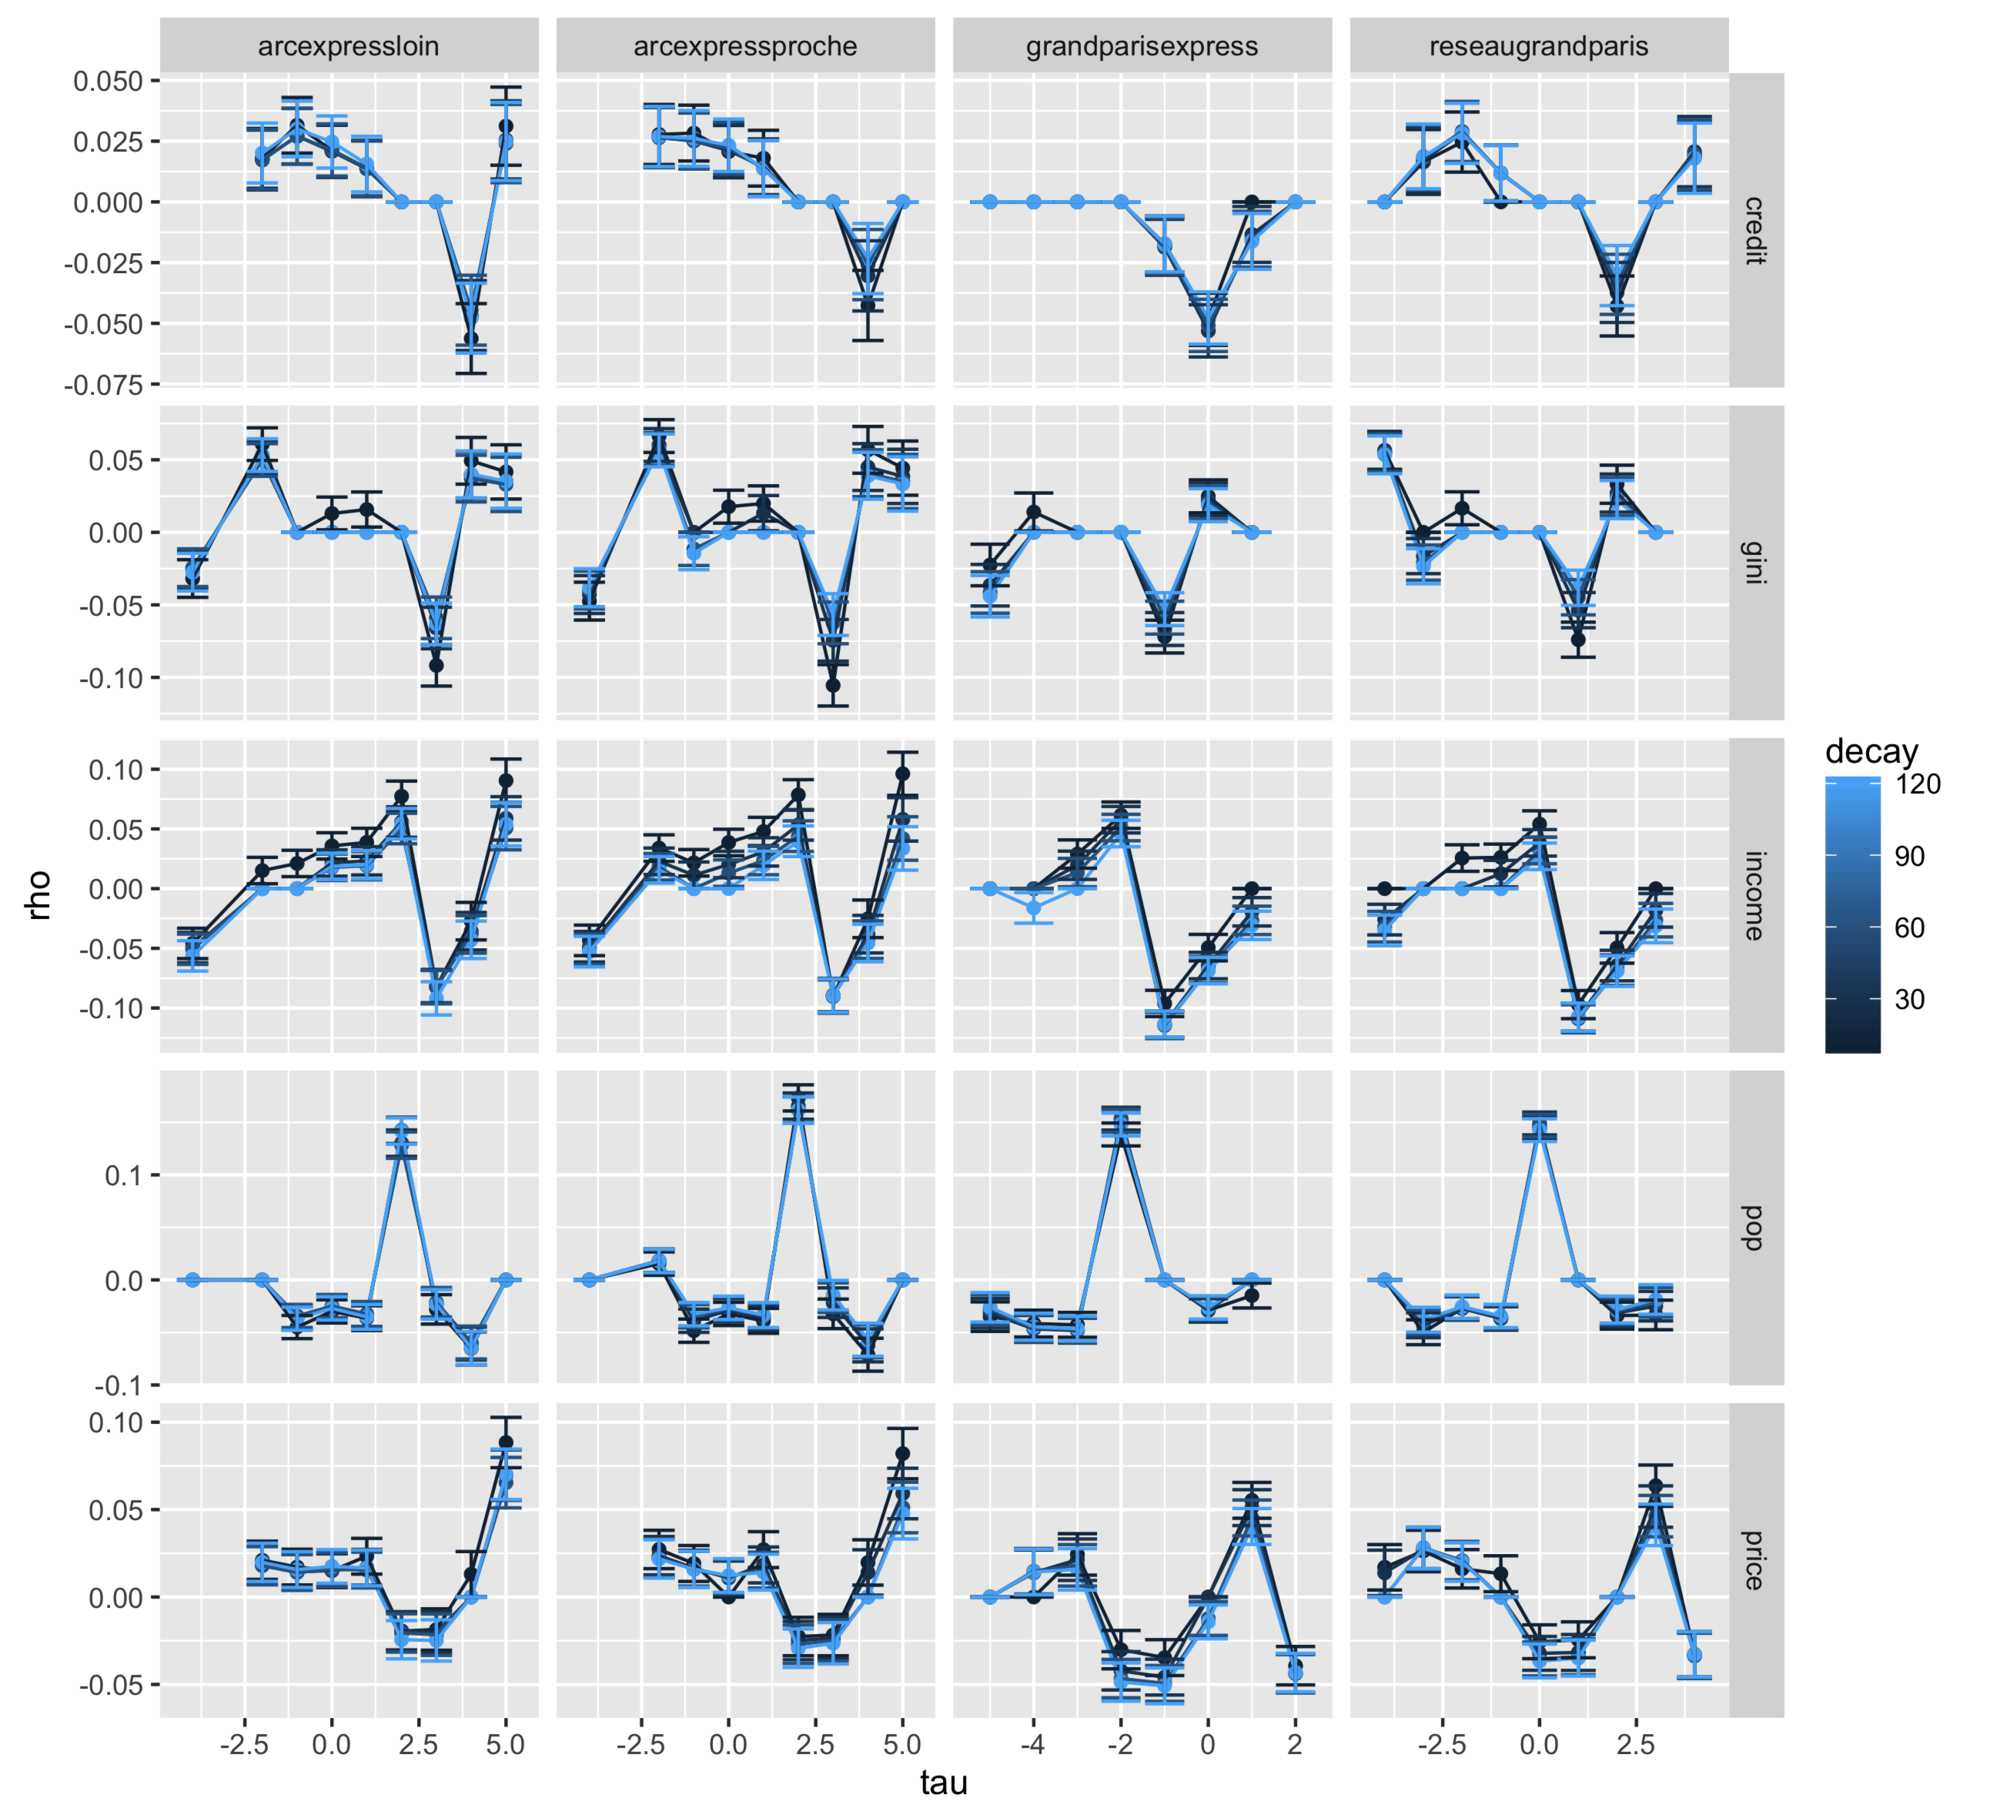
\includegraphics[width=\textwidth]{Figures/Final/1-2-1-fig-casestudies-empiricalres.jpg}
\caption[][Corrélations retardées empiriques]{\textbf{Empirical lagged correlations.} Plots show the value of lagged correlation between accessibility differentials in average travel time $\Delta T$ for each project (in colunms) and socio-economic and real estate variables variations (in rows). All are computed for different values of the decay parameter (\texttt{decay}, given by curve color). Error bars give the 95\% confidence interval.\label{fig:empiricalres}}{\textbf{Corrélations retardées empiriques.} Les graphiques donnent la valeur de la correlation entre le différentiel d'accessibilité en temps de trajet moyen $\Delta T$ pour chaque projet (en colonnes) et le différentiel des différentes variables socio-economiques et de transactions immobilières (en lignes), pour différentes valeurs du paramètre d'atténuation (\texttt{decay}). Les barres d'erreur donnent l'intervalle de confiance à 95\%.\label{fig:casestudies:empiricalres}}
\end{figure}
%%%%%%%%%%%%%%%
















%-------------------------


%%%%%%%%%%%%%%%%%%%%%%%%
%\subsection[Pearl River Delta][Le Delta de la Rivière des Perles]{Pearl River Delta: new urban regimes and mega-city regions}{Le Delta de la Rivière des Perles : nouveaux régimes urbains et Mega-région urbaine}
\subsection{Pearl River Delta}{Le Delta de la Rivière des Perles}


\paragraph{New urban regimes and mega-city regions}{Nouveaux régimes urbains et Mega-région urbaine}

\bpar{}{
Si la notion de megalopolis peut être tracée jusqu'à \noun{Gottmann}~\cite{gottmann1964megalopolis}, et qu'elle est à l'origine de celle de \emph{Mega-city Region} (MCR) consacrée par \noun{Hall}~\cite{hall2006polycentric}, il est clair que cette dernière est toujours plus d'actualité avec l'apparition récente de nouveaux régimes, notamment par l'urbanisation accélérée dans des pays à forte croissance économique et en mutation très rapide comme la Chine~\cite{swerts2015megacities}. Le second cas que nous développons ici rentre dans cette catégorie : le Delta de la Rivière des Perles est une des illustrations classiques de la structure d'une MCR fortement polycentrique. Historiquement initialement composé de Guangzhou uniquement, le développement de Hong-Kong puis la mise en place Zones Economiques Spéciales (\cn{经济特区}) dans le cadre des politiques d'ouverture de \noun{Deng Xioaping}, a conduit à un développement extrêmement rapide de Shenzhen, et dans une moindre mesure de Zhuhai. La province du Guangdong dans lequel le PRD se situe intégralement a actuellement le plus fort PIB régional de Chine, et la MCR regroupe une population d'environ 60 millions (les estimations fluctuant fortement selon la définition prise de la MCR et la prise en compte de la population flottante). Le phénomène de migration des campagnes est très présent dans la région et une ville comme Dongguan a par exemple basé son économie sur des manufactures employant ces travailleurs migrants.
}


\bpar{}{
\cite{Ye2014200} analyse les actions de gouvernance métropolitaine à l'échelle de centres de la MCR, et plus particulièrement comment les communes de Guangzhou et Foshan ont progressivement accru leur coopération pour former une zone métropolitaine intégrée, pouvant ainsi fortement influencer le développement des transports par exemple et permettant la mise en place d'un réseau connecté. Une forte tension entre des processus émergents par le bas, et un dirigisme d'état relativement fort en Chine, se répercutant de l'Etat central, au gouvernement provincial jusqu'aux gouvernements locaux, a permis la mise en place d'une telle structure. La compétition avec les autre villes de la MCR reste très forte, et la logique d'intégration de la MCR est partiellement guidée par la région seulement. La nature particulière des ZES de Shenzhen et Zhuhai, liée aux relations privilégiées avec les Zones Administratives Spéciales de Hong-Kong et Macao, qui n'ont été réintégrées à la République Populaire qu'à la fin du millénaire et conservent un certain niveau d'indépendance en termes de gouvernance, complique encore les jeux d'acteurs au sein de la région. La question d'un niveau de gouvernance qui expliquerait tel ou tel processus urbain est épineuse : \cite{liao2017ouverture} interprète les transferts progressifs des initiatives économiques du pouvoir central vers les autorités locales comme une forme de gouvernance multi-niveau. Dans le cadre des transports pour la MCR, il n'existe pas d'autorité d'organisation des transports, et chaque commune gère indépendamment le réseau local, tandis que les connections entre villes sont assurées par le réseau de train national. Cela conduit à des situations particulières dans lesquelles des zones se retrouveront très enclavées, avec une hétérogénéité très forte localement. Ainsi, la pointe sud de la ville de Guangzhou qui sert d'accès direct à la mer, est plus proche géographiquement du centre de Zhongshan, mais un lien direct par transports en commun est difficile à envisager, alors que la zone est bien reliée au centre de Guangzhou par la ligne de métro. Une situation similaire s'observe au terminus de la ligne 11 de Shenzhen, pour le quartier limitrophe de Dongguan, ce dernier étant très peu accessible. Cette situation serait cependant transitoire, étant donné les infrastructures déjà en construction et celles planifiées sur un plus long terme : le métro de Shenzhen, qui couvre aujourd'hui 285km, est planifié jusqu'à 30 lignes et 1142km en 2030~\cite{shenzhen2016plan}. Il est clair que ces développements suivent pour la majorité un développement urbain existant, une question cruciale est la volonté et la capacité à contenir l'étalement urbain et structurer les futurs développements autour de ce nouveau réseau, dans l'esprit d'une intégration volontaire entre urbanisme et transport de type Transit Oriented Development. Différents terminus seront connectés au metro de Dongguan, et de nouvelles lignes intercités structureront les déplacements de plus longue portée, ce qui fera du Delta dans un horizon temporel proche une MCR relativement bien intégrée en termes de transports en communs.
}


\paragraph{Impact of the Zhuhai-Hong-Kong-Macao bridge}{Impact du Pont Zhuhai-Hong-Kong-Macao}

Un projet iconique d'infrastructure de transport dans la région est le pont fermant l'embouchure du Delta, reliant Zhuhai et Macao à Hong-Kong. En réalité un Pont-tunnel. La longueur de la traversée est de 36.5km, ce qui en fait un ouvrage d'art exceptionnel. L'ouverture au traffic a été retardée de plusieurs années et est prévue finalement pour fin 2017\footnote{voir \texttt{http://www.hzmb.org/cn/default.asp}}. \cite{zhou2016medium} montre que les changements de motifs d'accessibilité attendus pour l'Ouest du Delta sont relativement forts, et ceux-ci peuvent potentiellement induire de fortes bifurcations dans les trajectoires des villes. La nécessité du projet est supportée par une narration de fort bénéfice économique dans le cadre des politiques d'ouverture, ainsi que par un bénéfice social pour l'Ouest notamment. Par exemple, Zhuhai se positionne comme un nouveau pivot entre Hong-Kong et l'ouest. L'équilibrage d'accessibilité s'opère cependant pour le mode routier uniquement, ce qui conduit à questionner ses impacts potentiels : d'une part l'accès systématique à l'automobile reste réservé à une partie de la population seulement, d'autre part les externalités négatives de congestion peuvent rapidement modérer les gains d'accessibilité. Les impacts à moyen et long terme du pont sont ainsi difficile à estimer, une piste étant de poser le problème différemment et de chercher comprendre la dynamique du système métropolitain de manière intégrée, comme nous l'évoquerons en~\ref{sec:lutetia}.





%-------------------------


%%%%%%%%%%%%%%%%%%%%%%%%
\subsection{Comparability of case studies}{Comparabilité des études de cas}


La possibilité de transfert des modèles urbains est délicate, et la particularité Est-asiatique a déjà été montrée pour la structure économique, et comment celle-ci ne peut être interprétée de manière simple par une séparation des processus microscopiques et macroscopiques comme certaines lectures rapides et idéologiquement orientée ont pu le faire, comme la vision de la Banque Mondiale~\cite{amsden1994isn}. La comparabilité de systèmes urbains est une question ouverte au centre des enjeux de la Théorie Evolutive Urbaine, et est par exemple liée au caractère ergodique de ces systèmes : si la trajectoire d'une ville dans le temps capture l'ensemble des états urbains possibles, alors les différentes villes sont différentes manifestations du même processus stochastique à différentes périodes, et un ensemble de villes permettrait d'avoir une idée des trajectoires temporelles. Intuitivement ce n'est pas le cas, et la Théorie Evolutive postule en effet la non-ergodicité~\cite{pumain2012urban}, que nous étudierons plus en détail en~\ref{sec:staticcorrelations}.







\stars




